\section{Article Notes}
\subsection{Thermochromism}
\cite{intelligentWindows} 
\textbf{Intelligent Themochromic Windows} \\
The use of air-conditioning systems to maintain comfortable working and 
living environments has become more common [1]. This leads to an increase in hte use
of electricity and a concurrent increase in carbon dioxide emmissions and other 
atmospheric pollutants formed in the electricity generation process. A self-propagating cucle results,
in which blobal warming due to increases in these greenhouse gases necessitates the increased 
use of air conditioning systems. Technology is thus required that can reduce the use of air conditioning
commercial and residential buildings to help break this cycle. \\
\\
(...) window coatings can reduce cooling costs or heating requirements [2]. 
Using thermochromic coatings as intelligent window coatings[1-7], which change
their optical properties with temperature; usually related to a structural pase change on passing through a 
critical temperature $T_c$. Thermochromic coatings would be applicable to climates where there are extreme 
changes in temperature over the year, for example, central and northern Europe, Japan, the United States, 
and Canada, which have hot summers and cold winters. \\
\\
Vanadium(IV) oxide; transition temperature $Tc = 68 ^{\circ}$C; visually and infrared trasnparent belov $T_c$ 
$\rightarrow$ solar radiation passes through, keeping the interior warm. Below $T_c$ it becomes infrared reflective
and preventing excessive heating, while remaining visually transparent.\\
\\
Critical temperature for vanadium is too high, but this can be lowered to $25^{\circ}$C uing dopants ([9]),
most efficiently with tungsten(loading of only 2 atom percent required), in thin films prepared by physical 
vapor deposition methods [10] and sol-gel spin or dip coating [11]. \\
\\
problem: low luminous transmittance of the glazing VO$_2$ film [10-13]. (could be solved with doping[4]
or anti-reflective coating ([12])). Also one needs a method where the thin films of the material
can be applied cheaply and efficiently to the glass ([17]).\\
\\
(p.394) Discussion of MST(metal-to-semiconductor transition) of VO$_2$ and structure 
changes through the MST. Discussion involves structure figures.\\
\\
Goodenough proposes antiferroelectric transition being the drivings force
for the MST in VO$_2$. $\rightarrow$ two transition temperatures: one due to antiferroelectric
distortion and one due to the crystallographic distortion. \\
\\
The next paragraph explains how doping of various elements varies the MST temperature. 
The most effective dopant in reducing the temperature is Tungsten (additional info about tungsten 
and after that it considers other dopants). \\
\\
Thinner thickness, stress and strain can also reduce the thermchromic transition temperature.\\
\\
A little bit on VO$_2$ thin film durability? \\
Methods of preparing Pure  and doped Vanadium(IV) Oxide Films:\\ 
Sol-Gel Method: forming thin films by dip- or spin-coating substrates with solutions of metal alkoxides. \\
PVD Method: energetically removing atoms/molecules under reduced pressure conditions, then to react with seed gas. \\ 
CVD method: chemical vapor deposition, in particular atmospheric pressure CVD (APCVD). \\
APCVD: deposit tin solid films from gaseous precursors onto a suitable substrate. (+Pictorial representation)\\
(and more on APCVD).\\
\\
Comparison of the above methods. \\
\\
3 atom percent tungsten(VI) $\rightarrow$ transition temperature reduced to $5^{\circ}$C.\\
1.9 percent $\rightarrow$ $29^{\circ}$C.\\
transition temperature decreases linearly with tungsten atom percent incorporation(Figure). \\
\\
Summary: intelligent TC glass with desired switch temperature($25-30^{circ}$C, obtainable using APCVD.
Mst of the problems regarding commercial use are solvable. Market in household, offices, factories and space
exploration.\\


\newpage
\cite{TCcommercialProducts} 
\textbf{Thermochromism in Commercial Products} \\
\begin{itemize}
\item Thermochromic liquid crystals: Periodicity between layers, PITCH, and constructive interference!. 
   TC liquid crystals can have a versatile range of colors and useful color changes bewteen -30 
   and 120$^{\circ}$C, often with very high temperature sensitivity. TC liquid crystals are only useful when
   they are in the liquid crystalline phase, which is a meso-phase (an intermediate phase of matter) between
   an isotropic liquid (high temperature) and crystalline solid (low temperature), which restricts the
   temperature range of theur applicability.
\item \textbf{Microencapsulation}: Defined as the coating of small solid particles, liquid droplets,
   or gas bubbles with a thin film or coating or shell material, and typical particle sizes are
   1 to 1000 $\mu$m ([20] Kirk-Othmer Encycloped. of chem. Tech. 4thEd). For three component organic mixtures,
   particle sizes are < 50 $\mu$m. \textbf{Micro encapsulation allows the additional advantage 
   of combinations of several narrow color ranges}, and very sharp color changes, 
      as well as protection of the coloring agent
   from the environment ([16] Nakasuji med flere. Chem.Abs.).
   \textbf{complex coacervation} and \textbf{interfacial polymerization} $\rightarrow$ processes to
   microencapsulate thermochromic materials! Also described! Nice to include if I use thin layer on my 
   granular film!
\item Smart window candidates: Fe$_3$O$_4$, FeSi$_4$, NbO$_2$, NiS, Ti$_2$O$_3$ and VO$_2$, which
   owe their temperature change to a semiconductor-to-metallic state transition 
   (aka \textbf{Mott transition temperature})
\end{itemize}



\newpage
\cite{TCqualitativeDescription} 
\textbf{A Qualitative Description of Thermochromism in Color Measurements} \\
\begin{itemize}
\item Wyszecki and Stiles stated ([2] color science), for TC transmitting filters, that the spectral
   transmittance curve at a given wavelength with a large positive slope usually dereases with increasing
   temperature. As a rule: steeper(positive) slope $\rightarrow$ greater temperature effect! \\
   The curve with negative slope is of minor importance, but often causes transmittance increase for
   increasing temperature (if it is important). \\
   \\
   Neutral samples (gray, white, black) did not exhibit TC, because their spectral reflectance curves
   have a small or no slope.
\item Assuming nonfluorescent, linear material which is "nice" with respect to polarization effects, then
   \begin{align*}
      1 = R_{\lambda} + A_{\lambda} + T_{\lambda}
   \end{align*}
   where, $R_{\lambda}$ is the reflectance, $A_{\lambda}$ is the absorbance and $T_{\lambda}$ is the
   transmittance of the sample.\\
   Considering \textbf{transmitting samples}, the intensity $I_{\lambda}$ transmitted through a 
   sample of thickness $d$ is given by
   \begin{align*}
      I_{\lambda} = I_{0 \lambda} e^{- \mu_{\lambda} d}
   \end{align*}
   where $\mu_{\lambda}$ is the absorption coefficient of the sample at wavelength $\lambda$.
   The optical density $D$ is then given by:
   \begin{align*}
      D = -\log(T_{\lambda}) = -\log(\frac{I_{\lambda}}{I_{0\lambda}}) = \mu_{\lambda} d \log e
      = \frac{\mu_{\lambda}}{\ln 10}
   \end{align*}
   For \textbf{opaque samples} there is no transmittance, but the optical density can be calculated
   from the reflected intensity $I_{R\lambda}$:
   \begin{align*}
      D_{\lambda} = -\log(\frac{I_{R\lambda}}{I_{0\lambda}}).
   \end{align*}
   The light reflected from the material is also exponentially attenuated, for opaque materials.
   Thus, $D=\frac{\mu_{\lambda}}{\ln 10}$ holds for reflected light if $d$ is the distance the
   reflected light has passed in the material.
\end{itemize}


\newpage
\cite{renewableSustainableEnergyRev}
\textbf{A Qualitative Description of Thermochromism in Color Measurements} \\
\begin{itemize}
\item
\end{itemize}

      
\newpage
\cite{Kamalisarvestani2013}
%\cite{coatingTechOfTCthinFilmSmartWindows}
\textbf{Performance, materials and coating technologies of thermochromic thin films on smart windows} \\
\begin{itemize}
\item A significant amount of energy is consumed to maintain thermal comfort in buildings, 
   a huge portion which is lost through windows. 
   smart windows obtained by thin films is the solution. The touchstone of performance 
   is the change in visible and infra-red transmission and reflectance!
\item A significant amount of the energy consumption in buildings are mainly due to HVAC (heating, ventilation 
   and air conditioning) devices, used to obtain thermal comfort,
   The building energy consumption in developed contries accounts for 20-40$\%$ of the total energy use.
   (including further details of US and China energy consumption). The building energy consumption is even more
   dominant in hot and humid regions, using one-third to half of the elextricity produced in some contries.
   Energy related carbon dioxide emmision. Motivates energy saving measures to reduce building energy losses and CO$_2$
   emissions.
\item Two approaches to increase energy efficieny (7-10)
   \begin{itemize}
      \item Active stratergies: improving HVAC systems and building lighting.
      \item Passive stratergies: improving the thermal properties of the building envelope (elementss
         separating the indoor from outdoor), i.e. thermal insulation to wall, cool coatings on roofs
                  and coated window glazings.
   \end{itemize}
\item Windows are known as one of the most energy inefficient components of buildings.(11) \\
      Improving the thermal performance of windows will result in reduced electricity costs 
      and less greenhouse gas emmissions. \\
      In addition to controlling transmitted IR radiation an ideal window should be capable 
      of sufficient transmission of visible light(12). \\
      Improving glazing characteristics of windows such as 
      thermal transmittance and solar parameters is the most 
      important criterion to be considered in building winows standards (14).
\item International and local standards related to energy and lighting performance of windows TABLE.
\item \textbf{Smart windows} defined as the type of windows that partially block the unwanted solar radiation.
   The energy performance can be improved by increasing heat gain in cold weather and 
   decreasing it in hot weather by adopting
   windows radiative and thermal properties dynamically (25). Adding a 
   controllable absorbig layer on teh surface of hte glass
   can change the optical properties of the glass by controlling the 
   incident solar heat flux(26). Therefore, smart windows
   lead to reduced HVAC.energy consumption, size and elecric demand of the building (11,27,28).\\
\item $\big($Low emissivity (low-E) coatings are spectrally selective films that are aimed to let the 
   visible light pass through and block the IR and UV-wavelengths which generally create heating(10).
   Typically, there are two types of these coatings: the tin oxide based hard coating and the 
   silver based soft coating with higher IR reflectance and lower transmittance. The visible transmittance
   of hard coatings can be boosted with anti-reflecting silicon dioxide (29). $\big)$
\item \textbf{The switchable reflective devices} (also called dynamic tintable windows) are categorized into
   \textbf{passive-} and \textbf{active systems}:
   \begin{itemize}
         \item Passive devices: the switching process is activated automatically in accordance 
            with the environmental conditions, e.g. temperature and heat in thermochromic windows.
         \item Actice systems: Require an external triggering mechanism to perform the modulation. For 
            instance, electricity is the actuating signal in electrochromic windows. The active
            switchable glazing systems offer supplementary options compared to the passive systems 
            whereas their dependenvy on power supply and wiring should be reckoned with as a drawback.
   \end{itemize}
\item Chromic material, liquid crystals and suspended particle windows are the three most common
   active controlled intelligent windows (11). 
   (Chromic materials $=$ electrochromic(active), gasochromic(active),
   photochromic and thermochromic.
\item Providing a see-through mode is a must in any application.
\item (p.356) The technology using liquid crystals in intelligent windows is called Polymer.
   Dispersed liquid crystals (PDLC).
\item Electrochromic windows and thermochromic windows demand the lowest cooling energy, where the former
   require less energy for lighting than the latter (69). \textbf{Figure 1 (24) (nice figure comparing 
   TC to the other chromic glazings together with clear glass, tinted glass and reflective glass) }.
\item \textbf{Thermochromic Windows}: \textbf{ALSO NOTE PAGE 357! ALOT OF NICE FIGURES!!!}\\
   Word originates from the Greek roots: "thermos" meaning warm or hot; and "Chroma" which means color.
   Generally TC materials change color in response to temperature variations.\\
   The TC thin film is initially in its monoclinic state(cold state) at lower temperatures (usually
   room temperature). Monoclinic materials behave as semiconductors, less reflective especially in 
   the near-IR (NIR) radiation. As the temperature becomes higher than a certain point, the TC material
   changes its nature from monoclinic to rutile state(hot state), where the material acts like a 
   semi-metal, reflecting a wide range of solar radiation (76). \textbf{FIGURE 3}
   The transition is called \textbf{metal to semiconductor transition (MST)}.
\item \textbf{Figure 4}, The majority of the heat gain in solar spectrum takes place at NIR range
   (800-1200 nm) (78-80). The red line(line 1) indicates the transmittance of a perfect
   TCW in cold state. Visible light should be transmitted and NIR should be reflected. Long wave radiation
   is also reflected back to indoor. This transmittance approach leads to reduction of solar heat gain and is 
   apt in nearly all climates. \\
   The blue line(line 2) indicates the tranmittance of a perfect TCW in its hot state. Visible
   and near infrared radiation are transmitted, while long-wave infrared is reflected to inside.
   This transmittance mode is suitable in low temperature climates where solar heat gain is desired.
   Therefore, in high temperatures, TCW reduce NIR and far-IR transmittance, while in low temperatures
   they allow these parts of solar adiation to pass (82), (Figure 5). \\
   The MST is fully reversible, co-occurred with large variations in electrical and optical 
   properties in NIR range (83). The MST temperature should decrease to near the ambient
   temperature. Doping metal ions into the lattice of TC materials can alter the transition temp(84,85).
   The size and charge (84,86,87) of dopant ion, film's strain (88,89) as well as the variations in
   electron carrier density are the determinant factors prevailing on the fall or rise of the transition
   temperature (90).
\item The \textbf{Ideal spectral behavior of TCW} is presented in \textbf{Table 3}. 
   %\begin{table}
      %\caption{The ideal optical performance of thermochromic windows (adapted from (91)).}
      %\hline
      %\textbf{State}    & \textbf{Monoclinic/cold (T<T_t)}    & \textbf{Rutile/hot (T>T_t)}    \\
      %\hline
       %Wavelength        & Visible   \t NIR  & Visible   \t NIR  \\
       %Transmittance (T) & 60\%-65\% \t 80\% & 60\%-65\% \t 15\% \\
       %Reflectance (R)   & 17\%      \t 12\% & 17\%      \t 77\% \\
      %\hline
   %\end{table}
   The visible transmission and reflectance should be equal on both sides of transition, 
   while the infra-red variations
   are from $0\%$ to $65\%$. The change in transmittance ($\Delta T \% $) and reflectance ($ \Delta R \% $)
   can be formulated as (92):
   \begin{align*}
   \Delta T \% &= ( T_{hot} - T_{cold} ) \cdot 100 \\
   \Delta R \% &= ( R_{hot} - R_{cold} ) \cdot 100
   \end{align*}
   where hot and cold denotes transmittance/reflectance at the hot and cold state respectively.
\item The most common TC material in TCWs is pure \textbf{vanadium dioxide}, with a transition temperature of
   $68  ^{\circ}$C which shoud be decreased to ambient temperature for practical use.\\
   The most critical weakness of VO$_2$ coatings is their low transmittance in the visible range.
   Many studies have reported values between $40 \%$ and $50 \%$, which is well below the acceptable
   value of $60 \%$ (93, 94). \textbf{Table 4} shows the reported values of transmittance and reflectance
   in the visible and IR range for VO$_2$.
\item Low energy-saving efficiency also limits the application of VO$_2$ coatings. The
   change in transmittance before and after the transmittion temperature $T_t$, at 2500nm, is
   known as the \textbf{switching efficiency} $\eta_T$ and is the benchmark of energy-saving efficiency.
   (?why? because of lighting?). This value is incluenced by doping(107,108), microstructure(80,95,109-111),
   \textbf{and film thickness (80,88)}. The most paramount factor among them is film thickness that affects
   the switching efficiency most significantly. However, increasing the film thickness has an adverse
   effect on $T_{vis}$. As observed from table 4, \textbf{the ideal film thickness is between 40 and 80 nm}.
\item Crucial Steps to overcome the limited application of TWCs:
   \begin{itemize}
      \item Suitable doping(reducing $T_t$ and improving $T_{vis}$)
      \item Appropriate Coating Technology
      \item Adding efficient anti-reflecting coating(to increase $T_{vis}$) (read next title in article)
      \item Reducing coating costs
   \end{itemize}



      
\end{itemize}

\begin{figure}[h!]
  \centering
   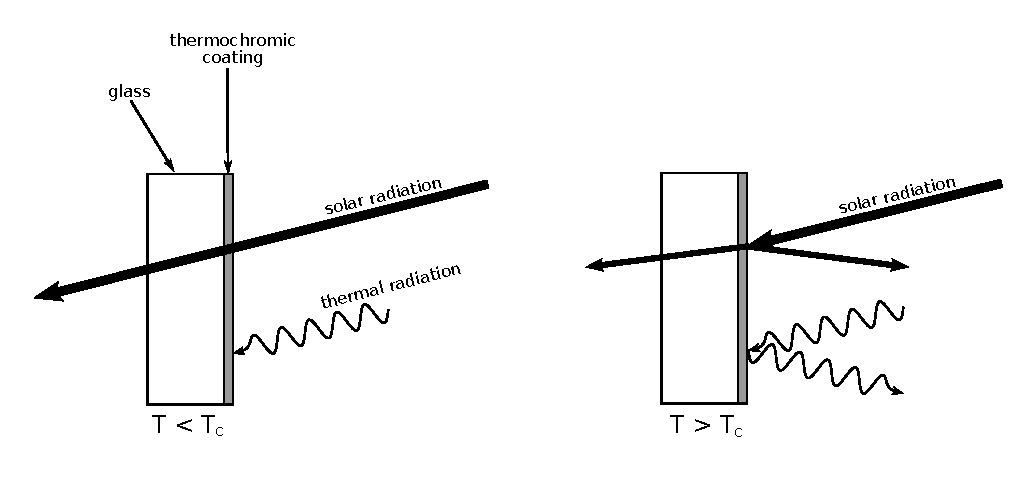
\includegraphics[width=0.5\textwidth]{../Figures/TCcoating.pdf}
   \caption{Schematic demonstration of the application of thermochromic materials to advanced window glazing [8].
   In the article it is used as a pictorial representation of how vanadium(IV) oxide thin film will work as 
   an intelligent window. }
\end{figure}


\clearpage
\begin{thebibliography}{9}

      \bibitem{opticalProperties}
      D. Bedeaux, J. Vlieger, 
      \emph{Optical Properties of Surfaces}, 
      Imperial College Press, 
      London, 2001

      \bibitem{intelligentWindows}
      Parkin IP, Manning TD.
      \emph{Intelligent thermochromic windows}, 
      Journal of Chemical Education,
      London 2006;83(3):393. ?I DON'T KNOW WHAT 393 is!? what is it?


      \bibitem{TCcommercialProducts}
      White MA, LeBlanc M.
      \emph{Thermochromism in Commercial Products}, 
      Journal of Chemical Education,
      Canada, September 1999;76(9) ?IS THIS RIGHT? IS SOMETHING WRONG? DO I MISS SOMETHING?!

      \bibitem{TCqualitativeDescription}
      Hiltunen J, Silfsten P, Jaaskelainen T, Parkkinen JPS,
      \emph{A Qualitative Description of Thermochromism in Color Measurements}, 
      ???????????????,
      ???????????????
      
      %\bibitem{Kamalisarvestani2013}
      %Kamalisarvestani M, Saidur R, Mekhilef S, Javadi FS,
      %\emph{Performance, materials and coating technologies of thermochromic thin films on smart windows}, 
      %Renewaable and Sustainable Energy Reviews 26 (2013) 353-364 ???????/????????   Elsevier?
      %Kuala Lumpur, Malaysia 2013; ???????????+

\end{thebibliography}

